\question{Магнитные линзы}

Фокусное расстояние магнитной линзы может быть определено интегрированием
уравнения траектории движении электронов в магнитном поле \eqref{eq11.2.57} и
\eqref{eq11.2.60}
\begin{equation}
  \left\{
    \begin{array}{l}
      \displaystyle r'(z_b) - r'(z_a) = -\abs{\frac{e}{m}}\frac{r_0}{8U_0}
        \int\limits_{z_a}^{z_b} B_0^2(z)\,dz; \\
      \displaystyle \phi_b - \phi_a = \sqrt{\abs{\frac{e}{m}}\frac{1}{8U_0}}
        \int\limits_{z_a}^{z_b} B_0(z)\,dz.
    \end{array}
  \right.
  \label{eq15system}
\end{equation}

Считая, что в области линзы траектория электронов изменяется мгновенно, имеем
\( r'(z_b) = -\tg\beta \) (рис.~\pic{15path}); а так как мы рассматриваем тонкую
линзу, то область в которой \( B_0 \ne 0 \) очень мала и можно изменить пределы
интегрирования на бесконечные. Тогда оптическая сила линзы:
\[
  \frac{1}{f_b} = \abs{\frac{e}{m}}\frac{1}{8U_0} \int\lii B_0^2(z)\,dz.
\]

Проделывая те же выкладки для электронов, вылетающих из области изображения,
получим, что
\[
  \frac{1}{f_a} = \abs{\frac{e}{m}}\frac{1}{8U_0} \int\lii B_0^2(z)\,dz =
    \frac{1}{f_b} = \frac{1}{f}.
\]

Угол поворота траектории электрона определяется из второго уравнения системы
\eqref{eq15system}.

\begin{figure}[h!]
  \center
%  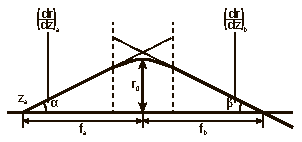
\includegraphics[width=.35\textwidth]{15_path} \hspace{1em}
%  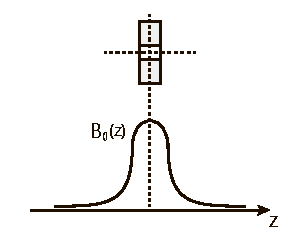
\includegraphics[width=.35\textwidth]{15_lens} \\
  \parbox{.35\textwidth}{\caption{Траектория электрона в поле короткой магнитной
    линзы} \label{pic15path}} \hspace{1em}
  \parbox{.35\textwidth}{\caption{Тонкая магнитная линза и распределение
    магнитной индукции на оси системы} \label{pic15lens}}
\end{figure}

Тонкая магнитная линза образуется короткой катушкой (рис.~\pic{15lens}),
создающей симметричное относительно центральной плоскости распределение
магнитного поля.

Оптическая сила такой линзы всегда положительна, то есть линза всегда собирающая
и не зависит от направления вектора магнитной индукции.

Поворот изображения зависит не только от величины, но и от направления и от
длины линзы, при этом изображение поворачивается целиком, так как угол поворота
не зависит от \( r \) и \( r' \).
